\documentclass{ximera}
%\usepackage{todonotes}

\usepackage{tkz-euclide}
\usetikzlibrary{backgrounds} %% for boxes around graphs
\usetikzlibrary{shapes,positioning}  %% Clouds and stars
\usetkzobj{all}
\usepackage[makeroom]{cancel} %% for strike outs
%\usepackage{mathtools} %% for pretty underbrace % Breaks Ximera
\usepackage{multicol}


\newcommand{\RR}{\mathbb R}
\renewcommand{\d}{\,d}
\newcommand{\dd}[2][]{\frac{d #1}{d #2}}
\renewcommand{\l}{\ell}
\newcommand{\ddx}{\frac{d}{dx}}
\newcommand{\zeroOverZero}{$\boldsymbol{\tfrac{0}{0}}$}
\newcommand{\numOverZero}{$\boldsymbol{\tfrac{\#}{0}}$}
\newcommand{\dfn}{\textbf}
\newcommand{\eval}[1]{\bigg[ #1 \bigg]}
\renewcommand{\epsilon}{\varepsilon}
\renewcommand{\iff}{\Leftrightarrow}

\DeclareMathOperator{\arccot}{arccot}
\DeclareMathOperator{\arcsec}{arcsec}
\DeclareMathOperator{\arccsc}{arccsc}


\colorlet{textColor}{black} 
\colorlet{background}{white}
\colorlet{penColor}{blue!50!black} % Color of a curve in a plot
\colorlet{penColor2}{red!50!black}% Color of a curve in a plot
\colorlet{penColor3}{red!50!blue} % Color of a curve in a plot
\colorlet{penColor4}{green!50!black} % Color of a curve in a plot
\colorlet{penColor5}{orange!80!black} % Color of a curve in a plot
                                      \colorlet{fill1}{blue!50!black!20} % Color of fill in a plot
\colorlet{fill2}{blue!10} % Color of fill in a plot
\colorlet{fillp}{fill1} % Color of positive area
\colorlet{filln}{red!50!black!20} % Color of negative area
\colorlet{gridColor}{gray!50} % Color of grid in a plot

\pgfmathdeclarefunction{gauss}{2}{% gives gaussian
  \pgfmathparse{1/(#2*sqrt(2*pi))*exp(-((x-#1)^2)/(2*#2^2))}%
}



\newcommand{\fullwidth}{}
\newcommand{\normalwidth}{}



%% makes a snazzy t-chart for evaluating functions
\newenvironment{tchart}{\rowcolors{2}{}{background!90!textColor}\array}{\endarray}

%%This is to help with formatting on future title pages.
\newenvironment{sectionOutcomes}{}{} 

\author{Emma Smith Zbarsky}
\license{Creative Commons Attribution 3.0 Unported}
\acknowledgement{https://quadbase.org/questions/q14526v1}
\begin{document}

\begin{exercise}

Find, and identify, the local extrema of
$g(x) = \frac{1}{5}x^5-\frac{2}{3}x^3+x-10.$


\begin{hint}
This is a problem of identifying extrema. Find the critical points of
the function $g(x)$ and then use the second derivative test to determine
whether they are local maxima or minima.
\end{hint}


\begin{hint}
\begin{align*}
g'(x) &= x^4-2x^2+1 \\
0 &= (x^2-1)^2 \\
x^*_1 = 1&; x^*_2 = -1 \\
& \\
g''(x) &= 4x^3-4x \\
g''(1) &= 4-4 = 0 \\
g''(-1) &= -4-(-4) = 0 
\end{align*} Therefore, the second derivative test is inconclusive.
Checking the graph, we see that there are no local extrema for this
function: 

\begin{image}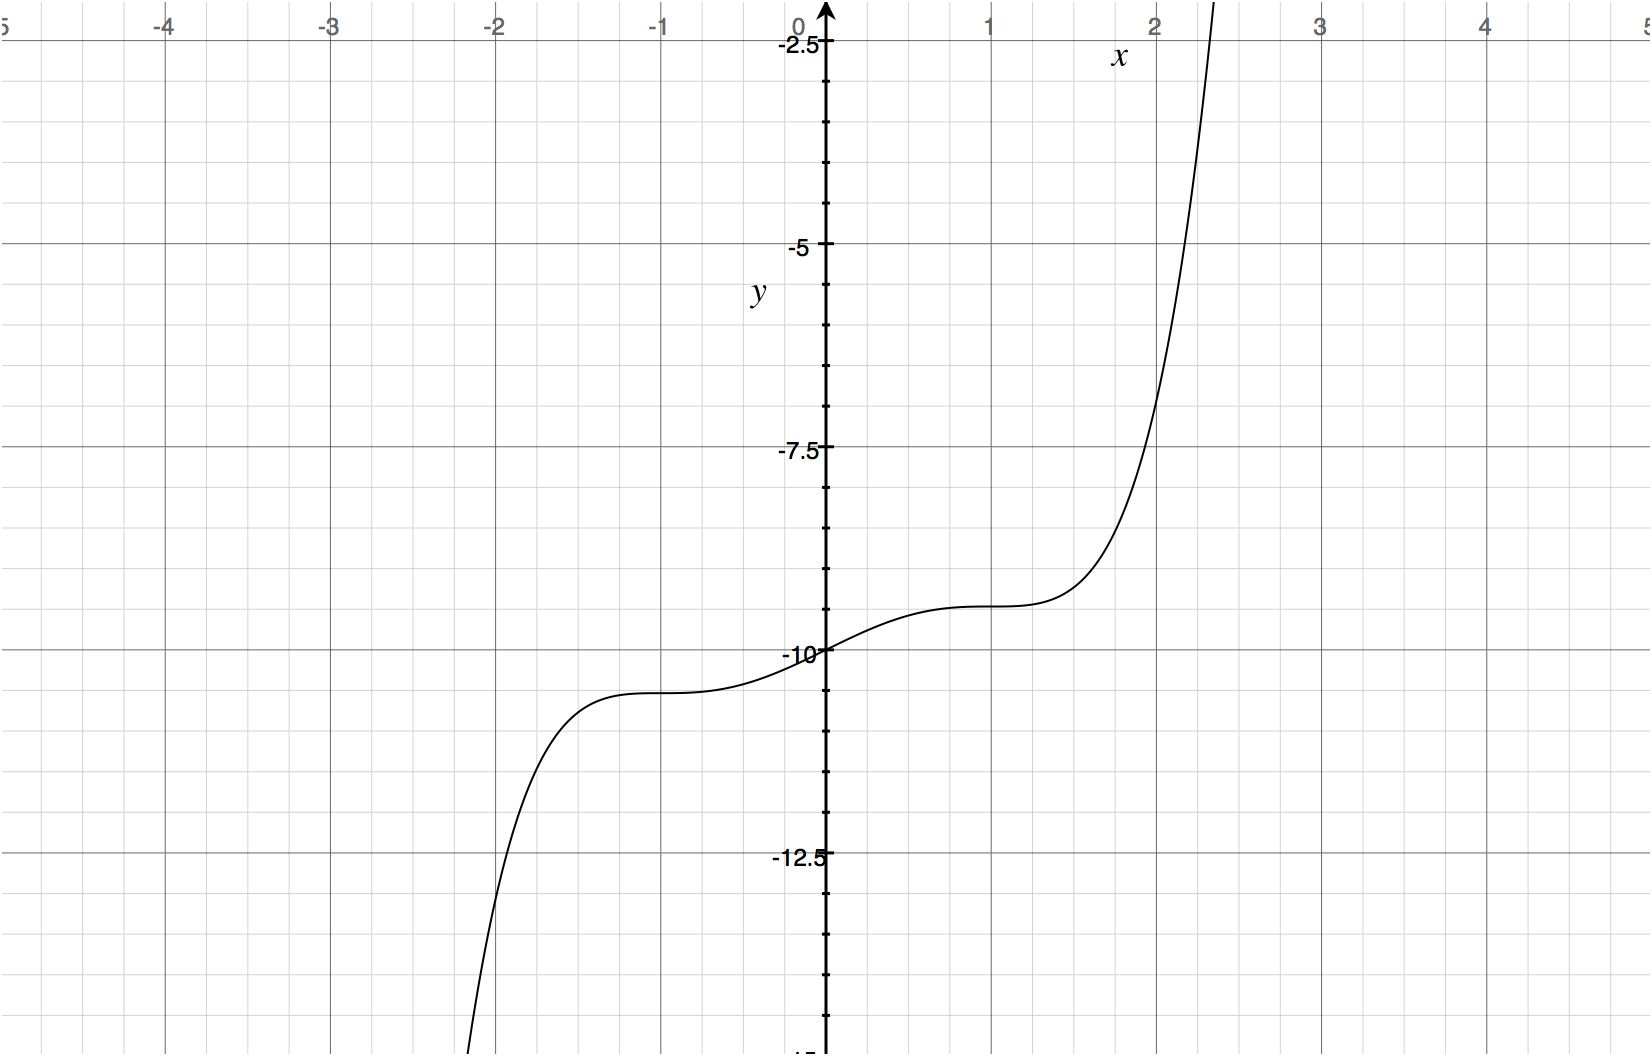
\includegraphics{extrema-none-graph.jpg}\end{image}
\end{hint}


\begin{multipleChoice}
\choice{There are two extrema:

\begin{itemize}
\item
  A maximum at $x=1$
\item
  A minimum at $x=-1$
\end{itemize}}
\choice{There are two extrema:

\begin{itemize}
\item
  A minimum at $x=1$
\item
  A maximum at $x=-1$
\end{itemize}}
\choice{There are four extrema:

\begin{itemize}
\item
  A minimum at $x=-2$
\item
  A maximum at $x=-1$
\item
  A minimum at $x=1$
\item
  A maximum at $x=2$
\end{itemize}}
\choice{There are four extrema:

\begin{itemize}
\item
  A maximum at $x=-2$
\item
  A minimum at $x=-1$
\item
  A maximum at $x=1$
\item
  A minimum at $x=2$
\end{itemize}}
\choice[correct]{The function $g$ has no extreme values.}
\end{multipleChoice}

\end{exercise}
\end{document}
